Docker hat den Grunsätzlichen Workflow von Build, Ship, Run. Wie ich das im Proof of Concept
gemacht habe, werde ich hier veranschaulichen.

\section{Build}

Um ein Image zu bauen kann man ein Dockerfile erstellen. meines sieht so aus:

\subsection{Dockerfile}

\begin{lstlisting}[
  captionpos=b,
  caption=Dockerfile,
  label=Dockerfile
]
  FROM java:8
  MAINTAINER Roman Wuersch

  COPY . /usr/src/yass
  WORKDIR /usr/src/yass

  EXPOSE 9090

  CMD ["./start-in-docker.sh"]
\end{lstlisting}

\begin{description}

\item[Zeile 1] Das Image leitet vom offiziellen OpenJDK 8 Image ab und baut darauf auf.

\item[Zeile 4] Kopiert alle Dateien im aktuellen Pfad ”.“ in das Image in den Pfad ”/urs/src/yass“. Das
sehe ich als eine der grössten Stärken an. Man kann sein Setup Lokal auf seiner Maschine so aufsetzten und testen
bis es alles sauber funktioniert und dann mit dieser Zeile genau den Inhalt in das Image replizieren.

\item[Zeile 5] Setzt das Startverzeichnis

\item[Zeile 7] Gibt an, dass der Port 9090 von einem Prozess verwendet wird und zukünftig angebunden werden kann

\item[Zeile 9] Der Befehl, welcher ausgeführt wird, wenn ein Container aus dem Image gestartet wird.

\end{description}

\subsection{Bauen via Shellscript}

Um das Image zu bauen habe ich ein Shell-Script gemacht:
\\

\begin{lstlisting}[
  captionpos=b,
  caption=Bauen eines Docker Images,
  label=BauenEinesDockerImages
]
#!/usr/bin/env bash
docker rmi -f sushicutta/docker-test
docker build -t sushicutta/docker-test .
\end{lstlisting}

Dieses Shell-Script sucht im aktuellen Verzeichnis ein Dockerfile und baut mit dessen
Angaben das Image.

\begin{description}

\item[Zeile 2] Löscht das bestehende Image sushicutta/docker-test aus dem Docker Hafen

\item[Zeile 3] Erstellt das Image neu unter dem selben Namen.

\end{description}

\section{Ship}

\subsection{Via Docker Hub}

Um das Image zu liefern, kann man nun Docker Hub verwenden.
\\

\begin{lstlisting}[
  captionpos=b,
  caption=Push to Docker Hub,
  label=PushToDockerHub
]
docker push sushicutta/docker-test
\end{lstlisting}

\subsection{Als .tar File}

Oder man kann das Image als .tar Datei speichern.
\\

\begin{lstlisting}[
  captionpos=b,
  caption=Docker Image exportieren,
  label=DockerImageExportieren
]
docker save -o docker-test.tar sushicutta/docker-test
\end{lstlisting}

Das gelieferte Image kann man dann irgendwo wieder importieren.
\\

\begin{lstlisting}[
  captionpos=b,
  caption=Docker Image importieren,
  label=DockerImageImportieren
]
docker load -i docker-test.tar
\end{lstlisting}

\subsection{Via SSH Tunnel}

Oder gleich das Image per SSH transportieren zippen und unzippen on the fly, und mit pv den
Pipe traffic darstellen:
\\

\begin{lstlisting}[
  captionpos=b,
  caption=SSH Transport mit zippen und network traffic Visualisierung,
  label=SSHTransport
]
docker save <image> | bzip2 | pv | \
     ssh user@host 'bunzip2 | docker load'
\end{lstlisting}

\section{Run}

Das Image ist jetzt gebaut worden und im Docker Hafen angekommen, und es trägt den Namen
sushicutta/docker-test.

Dieses Image kann nun beliebig viele Male gestartet werden.

Um das Image zweimal zu starten, benötigt man folgende Commands:
\\

\begin{lstlisting}[
  captionpos=b,
  caption=Image zwei mal starten auf den Ports 9091 und 9092,
  label=ImageZweimalStarten
]
docker run -d -p 9091:9090 --name yass-node-1 sushicutta/docker-test
docker run -d -p 9092:9090 --name yass-node-2 sushicutta/docker-test
\end{lstlisting}

Das Image läuft jetzt zweimal, der Inhalt ist zu 100\% identisch. Der unterschied
besteht darin, dass Docker nun den Ports 9091 des Host Betriebsystems auf den Port 9090 des
ersten Containers mapped und analog den Port 9092 des Host Betriebsystems auf den Port 9090
des zweiten Containers.

\begin{figure}[htbp]
  \begin{center}
    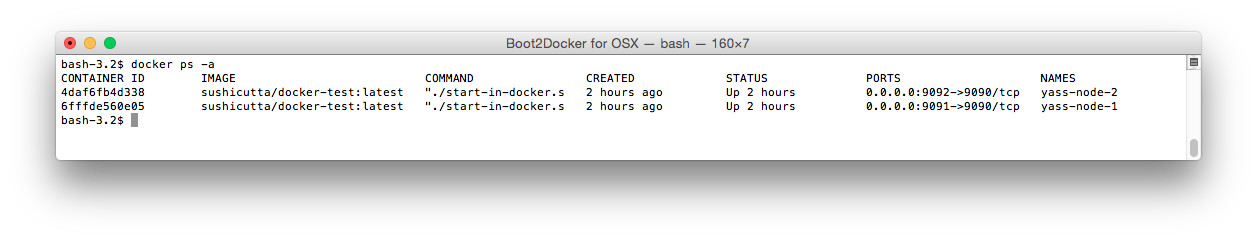
\includegraphics[width=1.0\textwidth]{./images/twoProcesses.png}
    \caption{Zwei identische Container auf verschiedenen Ports}
    \label{img:twoProcesses}
  \end{center}
\end{figure}

Was jetzt noch zum trägen kommt, ist der Start Befehl, der im Dockerfile
konfiguriert wurde. In unserem Beispiel start-in-docker.sh:
\\

\begin{lstlisting}[
  captionpos=b,
  caption=Start Script im Docker Container,
  label=StartScriptImDockerContainer
]
#!/usr/bin/env bash
java -Dfile.encoding=UTF-8 -classpath \
  "/usr/src/yass/lib/*:/usr/src/yass/build/classes/tutorial"\
  ch.softappeal.yass.tutorial.server.web.JettyServer 2>&1
\end{lstlisting}

Den Output der Prozesse kann man mit dem Befehl docker logs anschauen.

\begin{figure}[htbp]
  \begin{center}
    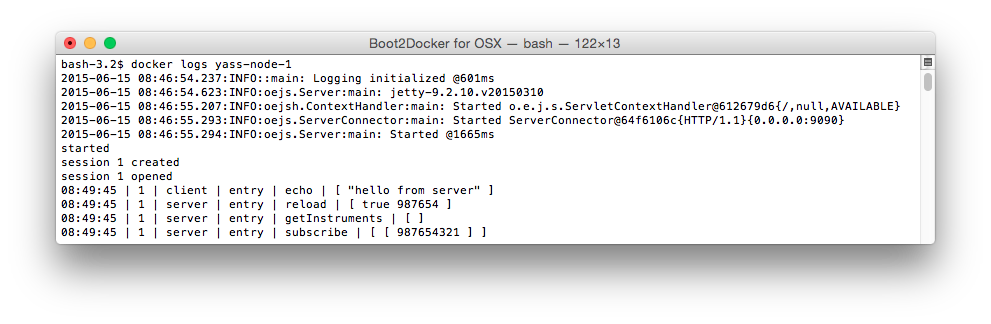
\includegraphics[width=1.0\textwidth]{./images/logOutput.png}
    \caption{Output am Stdout und Stderr sichbar machen vom Host Betriebsystem}
    \label{img:logOutput}
  \end{center}
\end{figure}





